\chapter{Transformer (2017)}

\begin{tcolorbox}
\fullcite{arxiv/1706.03762/Attention-Is-All-You-Need}
\end{tcolorbox}



\begin{enumerate}
    \item The (dominant) traditional sequence transduction models are based on complex recurrent or convolutional neural networks that include an encoder and a decoder.
    Some models also connect the encoder and decoder through an attention mechanism.
    \hfill \cite{arxiv/1706.03762/Attention-Is-All-You-Need}

    \item The Transformer, based solely on attention mechanisms, dispensing with recurrence and convolutions entirely. 
    \hfill \cite{arxiv/1706.03762/Attention-Is-All-You-Need}

    \item \textbf{Attention mechanisms} have become an integral part of compelling sequence modeling and transduction models in various tasks, allowing modeling of dependencies without regard to their distance in the input or output sequences.
    In all but a few cases, however, such attention mechanisms are used in conjunction with a recurrent network.
    \hfill \cite{arxiv/1706.03762/Attention-Is-All-You-Need}

    \item Transformer is a model architecture eschewing ($=$ avoiding) recurrence and instead relying entirely on an attention mechanism to draw global dependencies between input and output.
    \hfill \cite{arxiv/1706.03762/Attention-Is-All-You-Need}

    \item the number of operations required to relate signals from two arbitrary input or output positions (tokens) is a constant number of operations, albeit at the cost of reduced effective resolution due to averaging attention-weighted positions, an effect we counteract with Multi-Head Attention.
    \hfill \cite{arxiv/1706.03762/Attention-Is-All-You-Need}

    \item End-to-end memory networks are based on a recurrent attention mechanism instead of sequence-aligned recurrence and have been shown to perform well on simple-language question answering and language modeling tasks.
    \hfill \cite{arxiv/1706.03762/Attention-Is-All-You-Need}

\end{enumerate}





\section{Model Architecture (encoder-decoder)}

\begin{figure}[H]
    \centering
    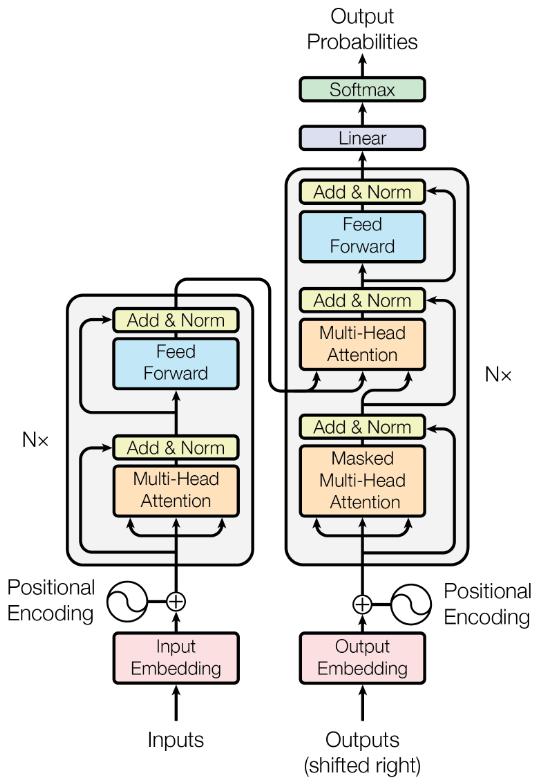
\includegraphics[
        width=\linewidth,
        height=10cm,
        keepaspectratio
    ]{images/advanced-ml/1706.03762v7.fig-1.transformer-arch.png}
    \caption*{
        Transformer - model architecture \\
        left - encoder, right - decoder
        \cite{arxiv/1706.03762/Attention-Is-All-You-Need}
    }
\end{figure}


\begin{enumerate}
    \item the encoder maps an input sequence of symbol representations $(x_1, \cdots, x_n)$ to a sequence of continuous representations $\bm{z} = (z_1, \cdots, z_n)$. 
    Given $\bm{z}$, the decoder then generates an output sequence $(y_1, \cdots, y_m)$ of symbols one element at a time. 
    At each step the model is auto-regressive, consuming the previously generated symbols as additional input when generating the next.
    \hfill \cite{arxiv/1706.03762/Attention-Is-All-You-Need}

    \item The Transformer follows this overall architecture using stacked self-attention and point-wise, fully connected layers for both the encoder and decode.
    \hfill \cite{arxiv/1706.03762/Attention-Is-All-You-Need}

    \item 
\end{enumerate}


\subsection{Encoder and Decoder Stacks}

\subsubsection*{Encoder}

\begin{enumerate}
    \item The encoder is composed of a stack of $N$ identical layers.

    \item Each layer has two sub-layers. 
    The first is a multi-head self-attention mechanism, and 
    the second is a simple, position-wise fully connected feed-forward network.
\end{enumerate}











\section{Self-Attention}

\begin{enumerate}
    \item Self-attention, sometimes called intra-attention is an attention mechanism relating different positions of a single sequence in order to compute a representation of the sequence. 
    \hfill \cite{arxiv/1706.03762/Attention-Is-All-You-Need}

    \item Self-attention has been used successfully in a variety of tasks including reading comprehension, abstractive summarization, textual entailment and learning task-independent sentence representation.
    \hfill \cite{arxiv/1706.03762/Attention-Is-All-You-Need}

    \item the self-attention mechanism allows every position to attend directly to every other position in a single step.
    \hfill \cite{common/online/chatgpt}

    \item That means any two tokens can interact in one operation, independent of how far apart they are in the sequence.
    \hfill \cite{common/online/chatgpt}

    \item the number of operations needed to connect two arbitrary positions is constant ($\mathcal{O}(1)$), not dependent on distance.
    \hfill \cite{common/online/chatgpt}

    \item Transformer is the first transduction model relying entirely on self-attention to compute representations of its input and output without using sequence-aligned RNNs or convolution. 
    \hfill \cite{arxiv/1706.03762/Attention-Is-All-You-Need}
\end{enumerate}






















